% Bagian: sets-functions-relations
% Bab: relations
% Subbagian: graphs

\documentclass[../../../include/open-logic-section]{subfiles}

\begin{document}

\olfileid[id]{sfr}{rel}{grp}
\olsection{Graf}

Sebuah \emph{graf} adalah diagram yang titik-titiknya dihubungkan oleh sisi.
Titik-titik tersebut disebut ``simpul'' atau ``verteks''. Graf merupakan alat
yang digunakan di
mana-mana dalam matematika diskret dan ilmu komputer. Graf sangat berguna
untuk merepresentasikan dan memvisualisasikan hubungan serta struktur, mulai
dari hal konkret seperti berbagai jenis jaringan hingga struktur abstrak
seperti kemungkinan hasil suatu keputusan. Literatur memuat banyak jenis graf
yang berbeda, misalnya menurut apakah sisinya berarah atau tidak, berlabel atau
tidak, apakah suatu simpul dapat mempunyai sisi menuju dirinya sendiri, apakah
dapat terdapat beberapa sisi di antara simpul yang sama, dan sebagainya.
\emph{Graf berarah} mempunyai hubungan khusus dengan relasi.

\begin{defn}[Graf berarah]
Suatu \emph{graf berarah} $G = \tuple{V, E}$ terdiri atas himpunan
\emph{simpul}~$V$ dan himpunan \emph{busur}~$E \subseteq V^2$.
\end{defn}

\begin{explain}
Menurut definisi kita, graf tidak lain adalah suatu himpunan beserta relasi
pada himpunan tersebut. Tentu saja, ketika membicarakan graf, wajar jika kita
mengharapkannya direpresentasikan secara grafis: kita dapat menggambar graf
dengan menghubungkan dua simpul~$v_1$ dan $v_2$ menggunakan panah jika dan
hanya jika $\tuple{v_1, v_2} \in E$. Satu-satunya perbedaan antara relasi saja
dan graf adalah bahwa graf menetapkan himpunan simpulnya; dengan kata lain,
graf dapat mempunyai simpul terisolasi. Namun, pokok pentingnya ialah bahwa
setiap relasi~$R$ pada himpunan~$X$ dapat dipandang sebagai graf berarah
$\tuple{X, R}$ dan, sebaliknya, graf berarah~$\tuple{V, E}$ dapat dipandang
sebagai relasi $E \subseteq V^2$ dengan himpunan $V$ yang dinyatakan secara
eksplisit.
\end{explain}

\begin{ex}
Graf $\tuple{V, E}$ dengan $V = \{1, 2, 3, 4\}$ dan $E =
\{\tuple{1,1}, \allowbreak \tuple{1, 2}, \allowbreak \tuple{1, 3},
\allowbreak \tuple{2, 3}\}$ tampak seperti berikut:
\begin{align*}
& 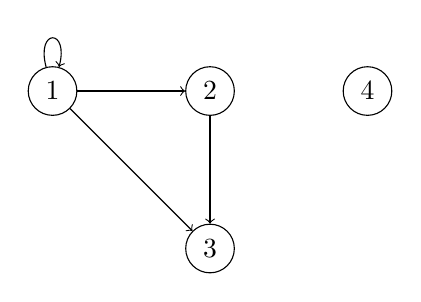
\begin{tikzpicture}[->,node distance=2cm]
  \node[draw,circle] (A) {$1$};
  \node[draw,circle] (B) [right of=A] {$2$};
  \node[draw,circle] (C) [below of=B] {$3$};
  \node[draw,circle] (D) [right of=B] {$4$};
  \draw (A) to [loop above]  (A);
  \draw (A) to  (B);
  \draw (A) to  (C);
  \draw (B) to  (C);
  \end{tikzpicture}
\intertext{Graf ini berbeda dari $\tuple{V', E}$ dengan $V' =
  \{1, 2, 3\}$, yang tampak seperti berikut:}
& 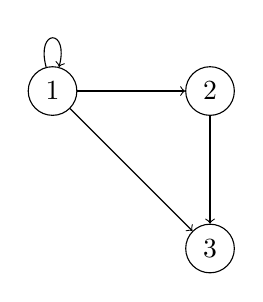
\begin{tikzpicture}[->,node distance=2cm]
  \node[draw,circle] (A) {$1$};
  \node[draw,circle] (B) [right of=A] {$2$};
  \node[draw,circle] (C) [below of=B] {$3$};
  \draw (A) to [loop above]  (A);
  \draw (A) to  (B);
  \draw (A) to  (C);
  \draw (B) to  (C);
  \end{tikzpicture}
\end{align*}
\end{ex}

\begin{prob}
  Pandang relasi lebih kecil daripada atau sama dengan~$\le$ pada himpunan
  $\{1, 2, 3, 4\}$ sebagai graf, lalu gambarkan diagram yang bersesuaian.
\end{prob}

\end{document}
